
We can say that the high nucleation rate in the beginning hints at some regions having more affinity than others and link to \cite{siahaan2022microtubule}

\begin{figure}[h!tb]
\centering
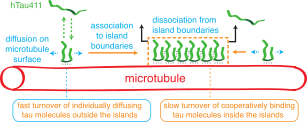
\includegraphics[scale=1]{Figures/tau8.png}
\caption[Schematic representation of island formation.]{
\textbf{Schematic representation of island formation.} Tau molecules bind and unbind with high rates to microtubules, on which they diffuse (fast turnover). When encountering an island (dashed orange box), tau molecules cooperatively associate with the island at its boundaries, rendering the tau molecules stationary, decreasing their unbinding rate (slow turnover), and causing the island to grow in size laterally. Tau molecules from solution can only bind to the inside of an island via displacement of an island-associated tau molecule, resulting in the observed concentration-dependent turnover of tau inside islands. After removal of tau from solution, tau molecules dissociate from the island boundaries, making the island shrink in size laterally.
	}\label{tau8}
\end{figure}
In our comprehensive investigation of tau interactions with microtubules, we have unveiled a complex and dynamic interplay between two distinct binding modes. This intricate relationship manifests in the formation of cohesive tau islands, a phenomenon that adds significant nuance to our understanding of tau's role in regulating microtubule-associated processes. Our findings, coupled with complementary work by \cite{tan2019microtubules}, paint a detailed picture of tau's multifaceted behavior on microtubules.
The cooperative binding mode, which we observed in the formation of tau islands, results in a population of stationary tau molecules characterized by remarkably low turnover rates. In stark contrast, we identified a diffusive mode comprising discretely binding tau molecules that exhibit high turnover rates. At physiological concentrations, these two distinct populations coexist on the microtubule surface. Intriguingly, the rapidly turning over tau has the potential to mask the underlying island structures, adding a layer of complexity to the visualization and study of these formations \aref{tau8}{}.
Our meticulous experiments revealed a characteristic density within tau islands of approximately 0.26 tau molecules per tubulin dimer. This consistent density strongly suggests the formation of an ordered monolayer, likely involving all four microtubule-binding repeats of tau. It's worth noting that recent cryo-electron microscopy studies have corroborated this density \parencite{Kellogg2018}, lending further support to our findings. However, it is crucial to highlight that the rapidly turning over tau population, which co-localizes with islands at physiological tau levels, remained elusive in these structural studies due to its highly transient nature.
The integrity of tau islands appears to hinge on cooperative interactions between the constituent molecules. This cooperativity could stem from direct tau-tau interactions, a hypothesis supported by previous studies demonstrating tau's propensity for liquid-liquid phase separation \parencite{HERNANDEZVEGA20172304} and its ability to form neurofibrillary tangles when hyperphosphorylated \parencite{iqbal2016tau}. Alternatively, or perhaps additionally, this cooperativity might arise from local tau-induced modifications of the microtubule surface. Such modifications could conceivably translate along the microtubule lattice to adjacent binding sites, thereby enhancing the affinity for incoming tau molecules.
A particularly intriguing observation from our study was that tau unbinding from islands increases with rising tau concentration in solution. Importantly, this phenomenon cannot be attributed solely to the rapidly turning over tau pool that co-localizes with islands at elevated concentrations. At 20 nM and 100 nM tau, this pool accounts for only approximately 20\% and 40\% of the total tau in the islands, respectively, while the average unbinding time drops by two orders of magnitude. We propose that this concentration-dependent unbinding results from the multivalent attachment of island-incorporated tau, mediated by its four microtubule-binding repeats and potential tau-tau interaction sites.
Our model suggests that these bonds undergo transient cycles of unbinding and rebinding. At low tau concentrations, transiently released bonds are likely reestablished as partially-bound tau molecules remain anchored to the microtubule by their persisting binding sites. However, with increasing tau concentration in solution, it becomes increasingly probable that a binding site of a solution-phase tau molecule establishes a bond to a temporarily-vacated binding site on the microtubule. This process could sequentially replace an island-incorporated tau molecule, one bond at a time. This concentration-dependent unbinding mechanism, previously reported for other multivalently interacting macromolecules \parencite{lanskydiffusible2015, sing2014multiple}, might also explain the kinesin-8-driven island disassembly we observed.
Our findings regarding the ionic strength dependence of island stability provide further support for the involvement of microtubule binding repeats in cooperative binding. We observed optimal stability at 75mM KCl, suggesting a delicate balance between hydrophobic interactions, likely mediated by the repeats, and ionic interactions. The stronger diffusive mode at 0mM KCl implies a predominance of ionic bonds in this binding mode. These ionic strength dependencies could also explain the varying stationarity of tau molecules within islands at different KCl concentrations. At lower KCl concentrations, single tau molecules within islands were less stationarily bound, potentially switching binding modes more frequently and often having only a subset of their microtubule binding repeats engaged.
The interplay between tau islands and motor proteins like kinesin-8 (Kip3) presents an intriguing regulatory mechanism. We can envision cycles of island growth, Kip3 traffic jam formation at island boundaries, eventual overwhelming and disassembly of the island by Kip3, propagation of the traffic jam as a high-density "pulse" along the microtubule, followed by island regrowth and repetition of the process. This dynamic interplay could potentially result in pulsatile Kip3 movement along axonal microtubules, adding another layer of complexity to cellular transport regulation.
Notably, we found that highly curved microtubule regions (radius < 2.5 µm) exhibited increased tau binding at low concentrations compared to surrounding areas, but lower than in islands on straight microtubule regions \pref{taucurve}{C,D}. Importantly, these highly curved regions were not protected from katanin-mediated severing \pref{taucurve}{G,H}, demonstrating that tau molecules in these areas do not form a cohesive layer. The binding of tau-mEGFP in curved regions was distinct from island formation on straight microtubules \pref{taucurve}{B}. These observations suggest that while high microtubule curvature attracts tau, it also prevents the formation of cohesive tau islands, potentially playing a role in regulating microtubule dynamics and interactions with other MAPs.
In conclusion, our study reveals that tau exists in two kinetically distinct phases on microtubules, forming cohesive islands through cooperative binding. This phenomenon may serve as a readout for post-translational tubulin modifications and influence the accessibility of microtubules to other MAPs. Furthermore, the potential for other intrinsically disordered proteins to form similar cohesive structures on microtubules could add another dimension to MAP sorting and regulation \parencite{Monroy2018}.
The implications of these findings extend to neurodegenerative diseases, where alterations in tau's ability to form islands, possibly due to hyperphosphorylation, could trigger various downstream pathophysiological effects. It is intriguing to speculate that in such diseases, diminished island assembly could cause a cascade of cellular disturbances. Future research should explore how these distinct tau phases interact with other cellular components, how their dysregulation might contribute to disease processes, and whether targeting these mechanisms could offer new therapeutic avenues for neurodegenerative disorders.